%resultados

Este Capítulo tiene como objetivo presentar los resultados obtenidos al realizar, desarrollar, construir e implementar (a escala prototipable) los diseños previamente concebidos en cada uno de los subsistemas del Capítulo anterior. 

\textbf{Nota: Es importante resaltar que aún cuando se tienen diseños y simulaciones, las circunstancias y limitantes hacen que se tomen nuevas consideraciones de diseño según corresponda.}

% ---XXX   Bitacora del tiempo de Buzz ligth year:  CAPITULO EN DESARROLLO 16/Noviembre/19   XXX---
% Tengo que ordenar las cosas, aquí están TEMPORALMENTE puestas asi a la maldita sea.
% HAY QUE ACLARAR QUE EN MEDIO DE UNA IMPLEMENTACIÓN HAY ALGO DE Diseño CORRECTIVO DE POR MEDIO (como una nota, observación o algo así) Y LUEGO SI YA ME PUEDO REGAR CON TODO LO HECHO COMO POR EJEMPLO LO DE LA CONEXIÓN DEL TORNILLO\\

\section{Subsistema de Identificación (ID)}
\subsection{Construcción del accesorio ``Jáquima RFID''}

La construcción del accesorio se realiza con la ayuda de impresoras 3D debido a su flexibilidad y disponibilidad en el Centro de Automatización de Procesos (CAP) de la Pontificia Universidad Javeriana Cali. Además, estas facilitan la obtención de productos físicos reduciendo costes de manufactura en elaboración de prototipos. El material utilizado para imprimir los diseños del accesorio es el filamento PLA de $1.75[mm]$.

% Una vez impresas las piezas, se obtienen resultados apreciables en la Figura \ref{jrfidpng}:

\begin{figure}
	\begin{center}
		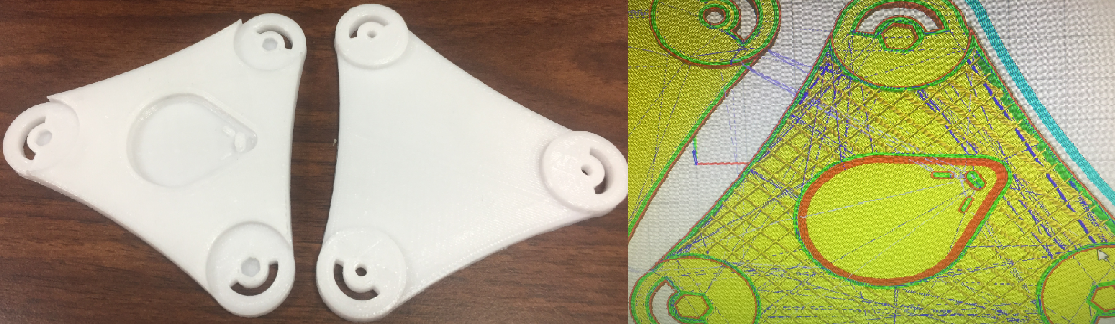
\includegraphics[scale=0.55]{img/jrfid.png}
	\end{center}
	\caption{Prototipo de accesorio RFID para la Jáquima. \label{jrfidpng}}
\end{figure}
\pagebreak

Se busca que los productos impresos hechos de este material estén en la capacidad de soportar impacto físico y permita el ensamblaje y des-ensamblaje de las piezas de manera efectiva. Con esto en mente se debe considerar un relleno o ``Infill'' entre 15 y 20\% de tipo línea; esto se observa gráficamente con la cuadrícula formada por el relleno mencionado (Ver lado derecho en la Figura \ref{jrfidpng}). De esta forma se garantiza una consistencia más resistente y robusta para este tipo de impresiones.

A comparación de las modalidades mencionadas en la Tabla \ref{matrizid}, este accesorio cuenta con las mejores características tal y como se puede apreciar en el diagrama radial mostrado en la Figura \ref{statsidpng}.

\begin{figure}[H]
	\begin{center}
		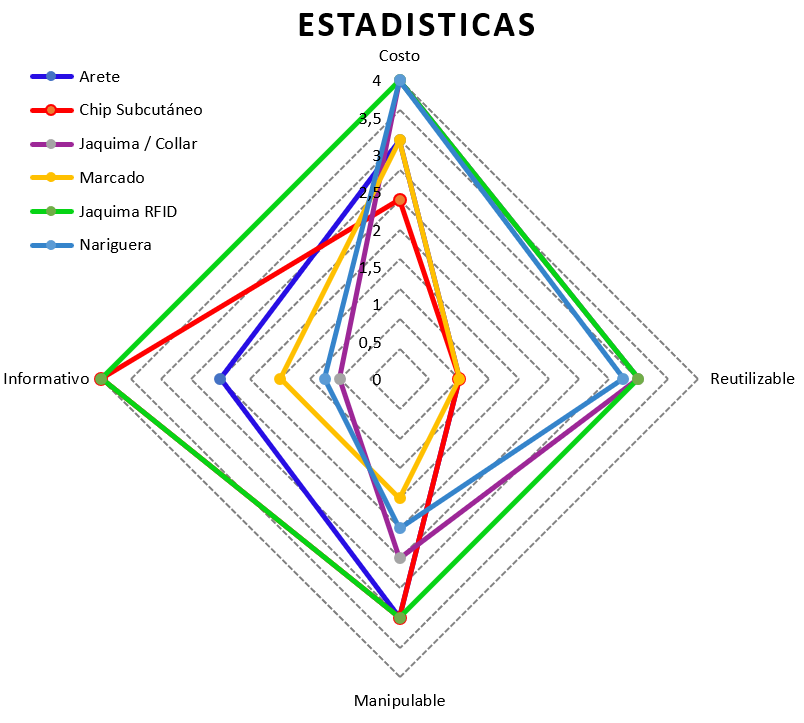
\includegraphics[scale=0.55]{img/statsid2.png}
	\end{center}
	\caption{Diagrama radial de las modalidades de identificación bovina. \label{statsidpng}}
\end{figure}

\subsection{Uso de la ``Jáquima RFID'' en campo}

En pro de mostrar un ejemplar de la Jaquima RFID se añade este accesorio a 2 bovinos de una finca ganadera ubicada en el municipio de Sotará (Cauca). La jáquima puede ser ajustada a reses de diferente tamaño y el accesorio RFID puede ser ajustado a la fisionomía variable del cráneo de estos animales (Ver Figura \ref{jarfidfinpng}).
\begin{figure}[H]
	\begin{center}
		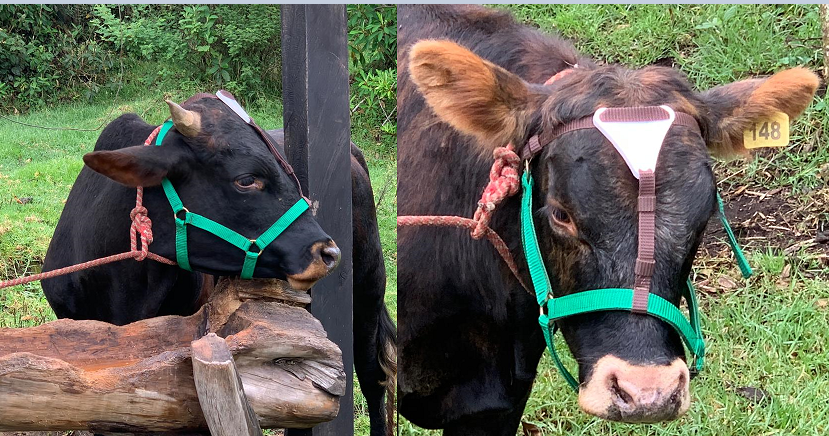
\includegraphics[scale=0.45]{img/jarfidfin.png}
	\end{center}
	\caption{Uso de la jáquima RFID en ejemplares de ganado. \label{jarfidfinpng}}
\end{figure}

\subsection{Resultados de la Identificación}

Para satisfacer de manera experimental el objetivo específico \#4, se logra la identificación del ganado de manera electrónica mediante el lector RFID MFRC522 conectado al Arduino tal y como se indica en la Tabla \ref{conexrfid} y como se muestra en la Figura a continuación.

\begin{table}[H]
\centering
\caption{Conexión de pines entre el lector RFID MFRC522 y el Arduino Mega.}
\label{conexrfid}
\begin{tabular}{|
>{\columncolor[HTML]{FFFFC7}}l |l|l|l|l|l|l|l|}
\hline
\textbf{Pin MFRC522} & 3.3V & GND & SCK & SDA & MISO & MOSI & RST \\ \hline
\textbf{Pin MEGA}    & 3.3V & GND & 52  & 53  & 50   & 51   & 5   \\ \hline
\end{tabular}
\end{table}

\begin{figure}[H]
	\begin{center}
		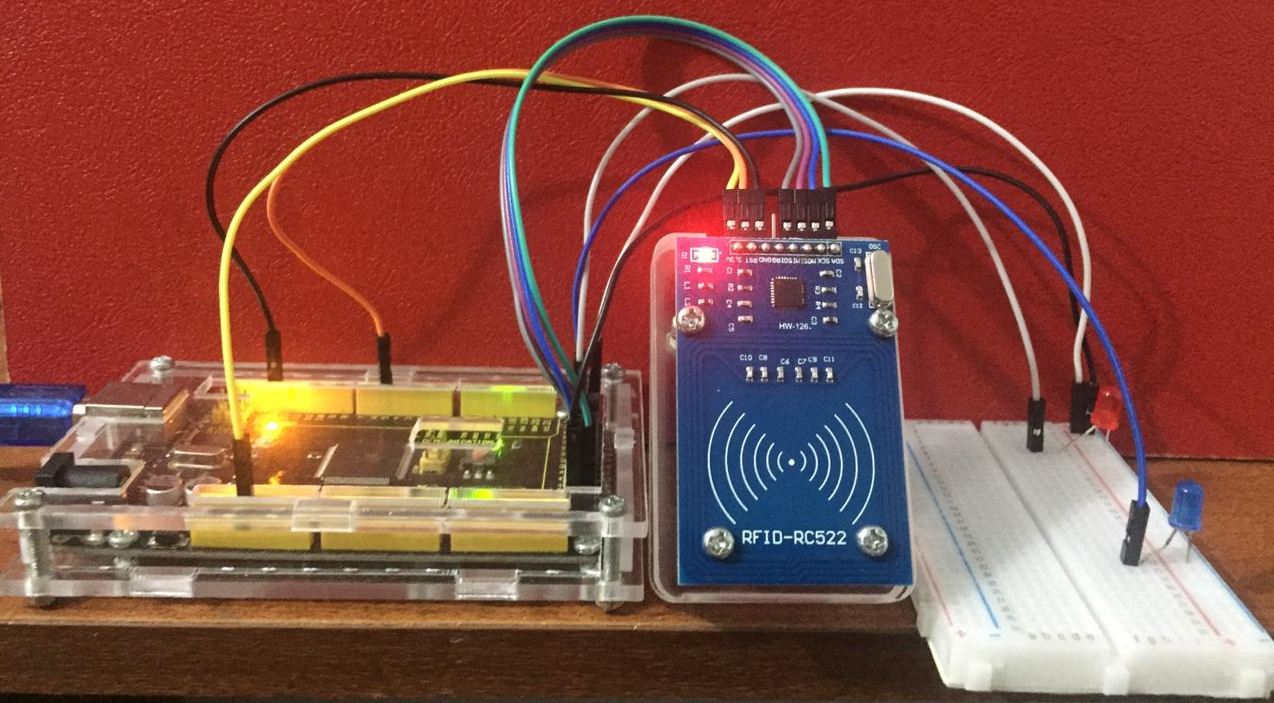
\includegraphics[scale=0.30]{img/rfidconarduino.png}
	\end{center}
	\caption{Conexión del modulo MRFC522 con un arduino Mega.}\label{conexrfidpng}
\end{figure}
\pagebreak

Una vez hechas las conexiones pertinentes, se utilizan ciertos comandos y librerías especiales para manipular el lector tal y como se describe a continuación:

\begin{figure}[H]
	\begin{center}
		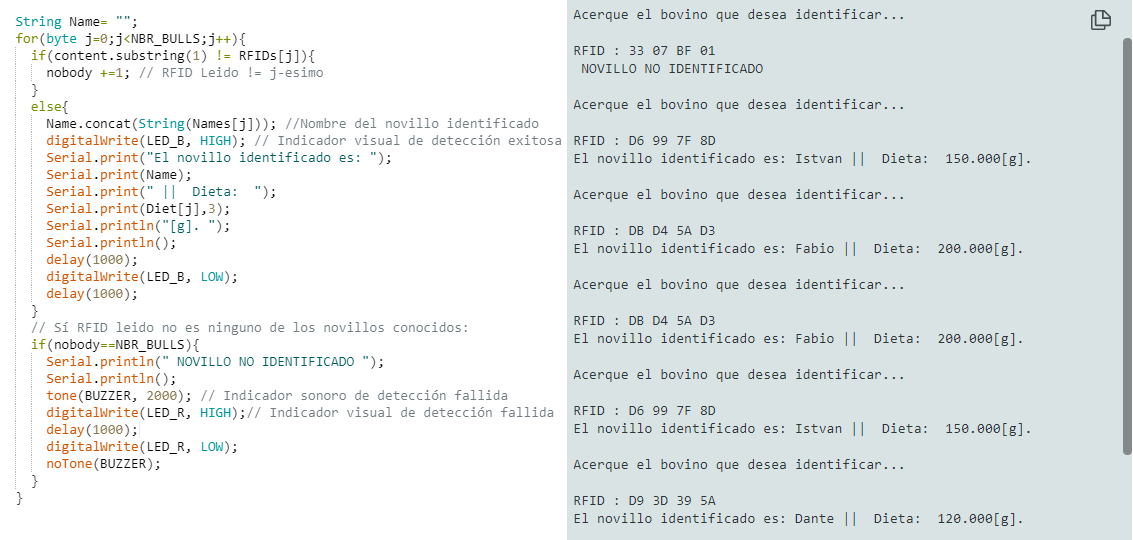
\includegraphics[scale=0.55]{img/cmdrfid.png}
	\end{center}
	\caption{Código y ejecución del programa de identificación de novillos.}
\end{figure}

En la Figura anterior se puede observar un fragmento del código que evidencia la lógica que permite identificar exitosamente a un novillo. Teniendo presente la Figura \ref{conexrfidpng}, en caso tal que se acerque una etiqueta RFID identificada, y por lo tanto asociada a un novillo, un LED de color azul indica visualmente que el novillo ha sido identificado satisfactoriamente; esto puede corroborarse en la parte derecha de la Figura anterior, al notar que se imprimen en pantalla el RFID identificado, el nombre del novillo correspondiente y su porción dietaria asociada. En caso contrario, el LED rojo de la Figura anterior indica que el novillo que se está intentando ingresar a un puesto de alimentación no está identificado, dando paso a la activación de una alarma visual y sonora; esto se corrobora en la Figura anterior al notar que se imprime en pantalla que el novillo acercado al lector no está identificado.

Otro caso de análisis es la verificación de novillos que ya han sido identificados con anterioridad y que por alguna razón desconocida han ingresado nuevamente al establo de alimentación. En este caso, cuando el novillo fue identificado y alimentado satisfactoriamente por primera vez, una variable cambia de cero (0) a uno (1), de esta forma cuando el novillo sea identificado nuevamente en una misma jornada de alimentación, se corrobora el valor de esta variable. En este punto, la variable poseerá un valor igual a 1, con lo que se puede afirmar que el novillo ya fue ingresado, identificado, y su alimento ha sido servido satisfactoriamente. Esta situación puede observarse en la Figura a continuación:

\begin{figure}[H]
	\begin{center}
		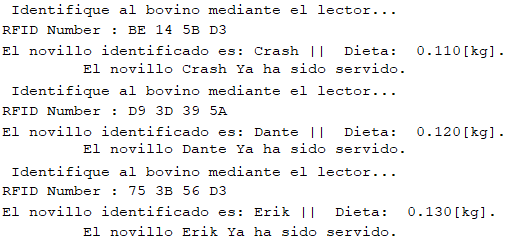
\includegraphics[scale=0.7]{img/reprfid.png}
	\end{center}
	\caption{Aviso textual del puerto Serial por reingreso de novillo previamente identificado.}
\end{figure}




\section{Subsistema de Estructura Mecánica}
\subsection{Forma de la tolva}

En el Capítulo anterior se describe la estructura mecánica de la tolva, haciendo referencia a un silo de almacenamiento. En pocas palabras, se requiere de un tanque cilíndrico con extremos cónicos para la entrada y salida del material. Por efectos de portabilidad y almacenamiento en condiciones de laboratorio, este elemento es construido a partir de piezas ensamblables de tubería PVC. 

Particularmente en el prototipo construido se utilizan 5 piezas distintas. En primer lugar, conexiones de tubería sanitaria de $6^{"}$ para conformar la parte cilíndrica de la tolva. En segundo lugar, se utilizan piezas de reducción de $6^{"}$ a $2^{"}$ para guiar la entrada y salida del material siendo estas las que conforman las partes cónicas de los extremos. Finalmente, la boquilla de entrada del material está compuesta por un accesorio de limpieza como el mencionado en la Sección \ref{} , con la cual se garantiza un almacenamiento reutilizable y hermético.

La tolva final del prototipo se observa en la Figura  \ref{tolvares}.

\begin{figure}[H]
	\begin{center}
		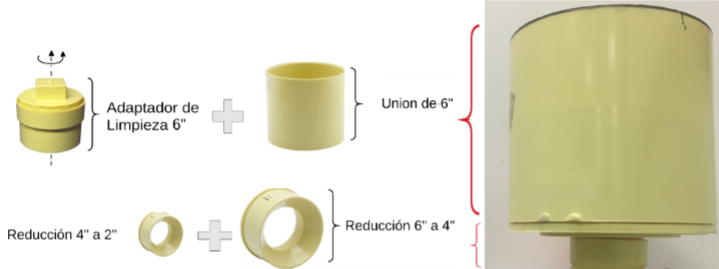
\includegraphics[scale=0.8]{img/tolvares2.png}
	\end{center}
	\caption{Composición final de la tolva del prototipo. \label{tolvares}}
\end{figure}

Las partes que conforman la tolva se pueden ver desde una vista superior (ver Figura \ref{vissuptolva})

\begin{figure}[H]
	\begin{center}
		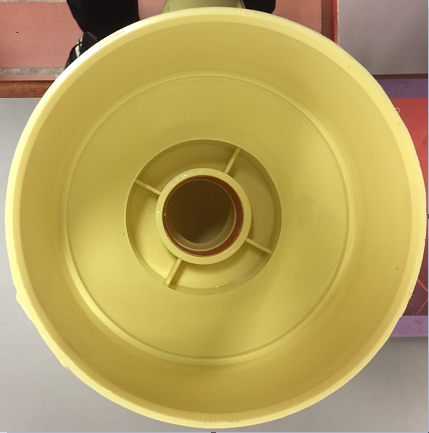
\includegraphics[scale=0.55]{img/vissuptolva2.png}
	\end{center}
	\caption{Vista superior: Composición interna de la tolva. \label{vissuptolva}}
\end{figure}

% \subsection{Distribución de los puntos de alimentación}
\subsection{Mecanismo de extracción: Tornillo sin fin}
\item \textbf{Construcción mecánica del tornillo sin fin}

Una vez llegados a este punto se procede a realizar la impresión 3D del tornillo diseñado en una de las impresoras 3D del CAP de la PUJC. No obstante se presentaron las siguientes dificultades:
    
\begin{itemize}
    \item La bandeja de impresión de las impresoras 3D del CAP sólo imprime objetos de dimensiones menores a $140[mm]$.
    \item La longitud del tornillo diseñado supera esas dimensiones.
    \item El tiempo de impresión supera las 24 horas.
    \item El material requerido para hacer la impresión supera el monto autorizado para estudiantes de la Carrera.
\end{itemize}
    
Estas limitaciones implican un rediseño del tornillo para que pueda ser impreso por lo que se toman las siguientes medidas:

\begin{itemize}
    \item El tornillo constará de 2 partes que al unirse conformarán el tornillo en su totalidad.
    % iguales que serán conectadas por 
    \item El diseño será modificado para que gaste menos material de impresión
    \item Al constar de diferentes piezas más pequeñas se reduce el tiempo de impresión por pieza, ajustándose a la demanda de impresión del CAP.
    \item La longitud del tornillo será igual, pero las piezas que lo conforman tendrán dimensiones menores a $140[mm]$.
\end{itemize}

Retomando la Figura \ref{accesoriograndepng}, el diseño de uno de los extremos del tornillo debe contener los orificios necesarios para realizar el acople entre el servo y el tornillo. Este diseño se puede apreciar a continuación:

\begin{figure}[H]
    \begin{center}
    	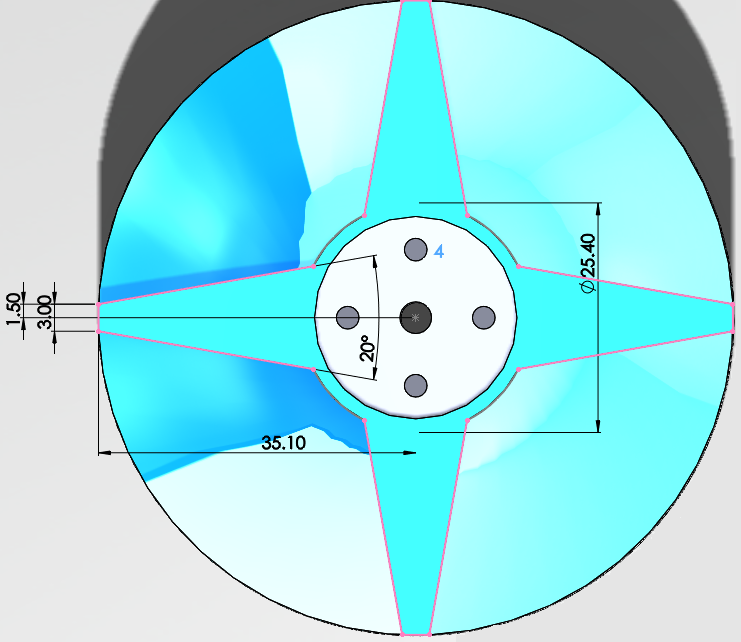
\includegraphics[scale=0.5]{img/motornillo.png}
    \end{center}
    \caption{Diseño del extremo del Tornillo que conecta con el servo motor. \label{motornillopng}}
\end{figure}
    
Ahora bien, dado que el tornillo constará de 2 partes, se debe considerar el modo de conexión. Para ello se opta por diseñar una parte tipo ``Macho'' y otra parte tipo ``Hembra''. De esta forma, el tornillo completo estaría formado por la conexión a presión de ambas partes.

\begin{figure}[H]
    \begin{center}
    	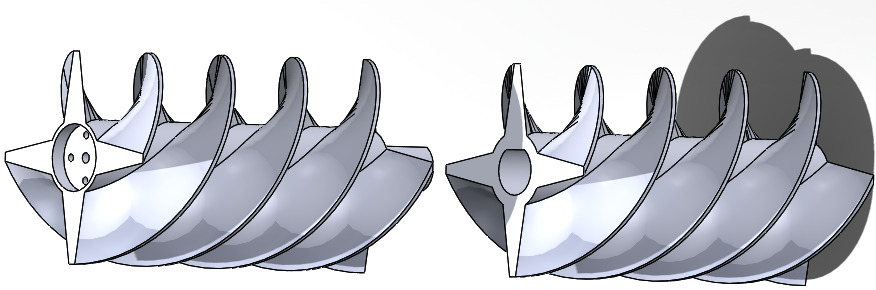
\includegraphics[scale=0.6]{img/semicircular.png}
    \end{center}
    \caption{Unión entre tornillos tipo ``Hembra'' y tipo ``Macho''. \label{semicircularpng}}
\end{figure}

Se había pensado que con la saliente semicircular del tornillo Macho sería suficiente para transmitir de manera apropiada el torque desde el servo hasta el extremo del tornillo. No obstante, el tornillo se ``desacoplaría'' en las condiciones en que el tornillo esté en su máxima capacidad de transporte, es decir cuando el tornillo esté transportando alimento desde su inicio hasta su fin. 

De esta forma se concluye que no se ejerce fricción suficiente entre las paredes internas del tornillo que bordean la saliente del tornillo Macho y de esta forma no se transmitiría de manera apropiada el torque desde el servo hasta el extremo final del tornillo.

Con base en lo anterior, se concluye que es necesario el uso de una $3^{era}$ pieza de conexión. Esta pieza deberá tener superficies planas que ayuden a la transmisión de torque. Por otra parte debe estar separado de ambos extremos por efectos de impresión y de calentamiento del material.\\

Siguiendo este orden de ideas, se resume lo siguiente:
\begin{itemize}
    \item El tornillo constará de 2 partes.
    \item La primera que conecta el servo junto con un extremo del tornillo
    \item La segunda que conecta, mediante una pieza extra, las 2 partes del tornillo.
    \item Ambas partes del tornillo serán de tipo ``Hembra''.
    \item La pieza de conexión contará con 2 orificios que servirán para pasar un seguro que mantendrá firme el acople de las 2 partes de tornillos con la pieza de conexión. (ver Figura \ref{piezaconexionpng})
    
    \begin{figure}[H]
        \begin{center}
    	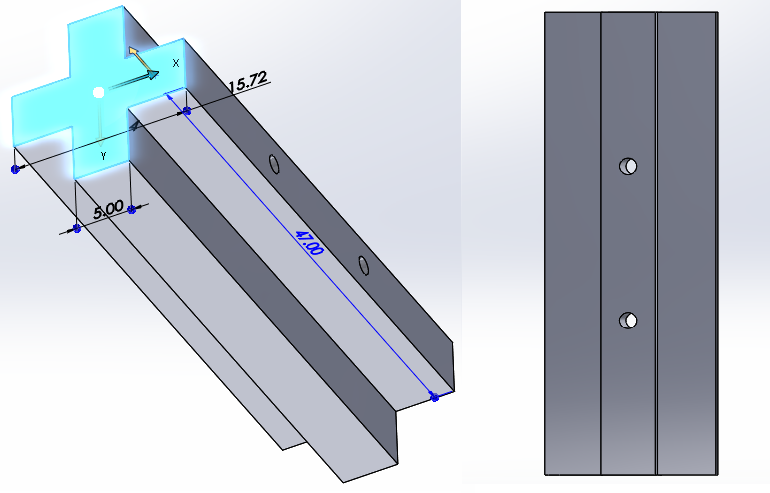
\includegraphics[scale=0.4]{img/piezaconexion.png}
        \end{center}
        \caption{Pieza auxiliar para conexión del Tornillo. \label{piezaconexionpng}}
    \end{figure}
    
    \item Ambas piezas de tornillo tipo Hembra tendrán un orificio sobre el eje principal basados en el ítem anterior.
\end{itemize}

En este punto se podría cuestionar la estructura interna del tornillo debido a la dificultad visual para asimilar el diseño del tornillo. Para ello se muestra el siguiente corte trasversal de la pieza de tornillo Hembra que conecta  con el servomotor (ver Figura \ref{cortetrasversalpng})

\begin{figure}[H]
    \begin{center}
    	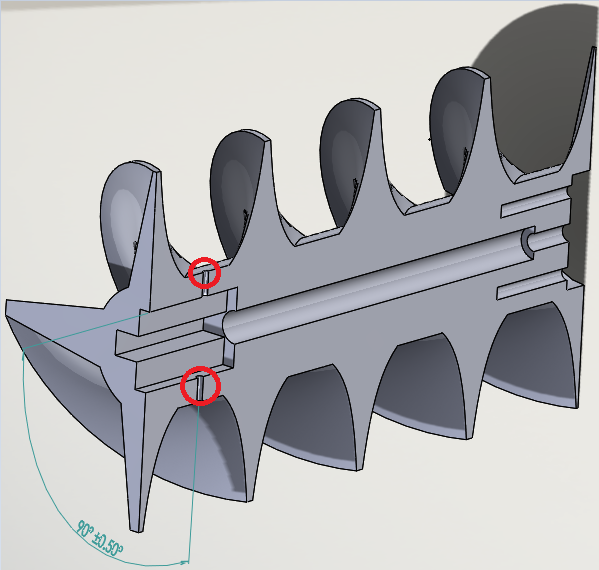
\includegraphics[scale=0.55]{img/cortetrasversal3.png}
    \end{center}
    \caption{Corte trasversal pieza tipo Hembra. \label{cortetrasversalpng}}
\end{figure}

\vspace{1mm}

En el lado izquierdo de la Figura \ref{cortetrasversalpng} se puede observar el espacio para unir la pieza de conexión y el seguro. En la parte media se puede observar el corte interno del tornillo por donde pasa el atornillador que fija el tornillo M3 al servo. Por último, en el lado derecho se observan los 4 orificios para atornillar el accesorio circular del servo a la pieza del tornillo. \\

Adicionalmente se puede observar la vista superficial de esta pieza tipo Hembra en la Figura \ref{vistainternapng}.

\begin{figure}[H]
    \begin{center}
    	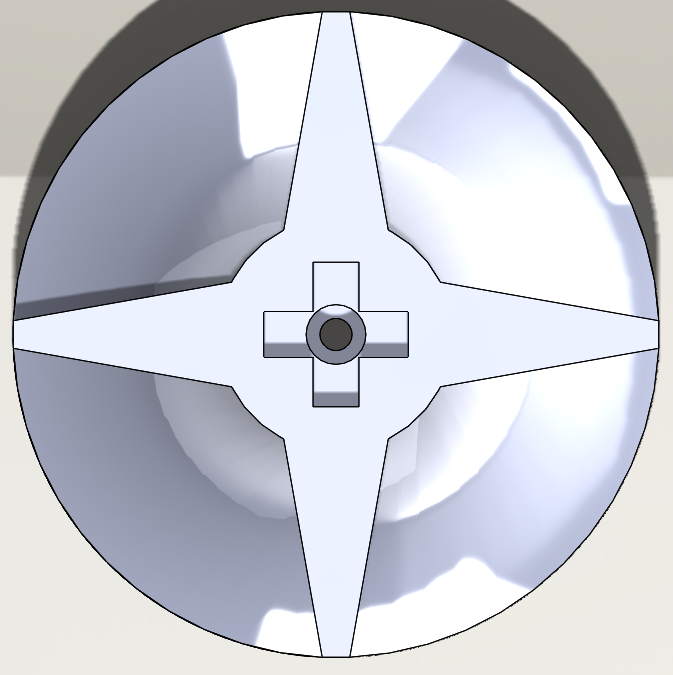
\includegraphics[scale=0.5]{img/vistainterna.png}
    \end{center}
    \caption{Vista interna de pieza tipo Hembra. \label{vistainternapng}}
\end{figure}

La composición final del tornillo consta del ensamblaje de las 2 piezas tipo hembra y el conector tipo cruz. El ensamblaje se logra al unir estas piezas como lo indica la Figura \ref{ensambletornipng}:

\begin{figure}[H]
    \begin{center}
    	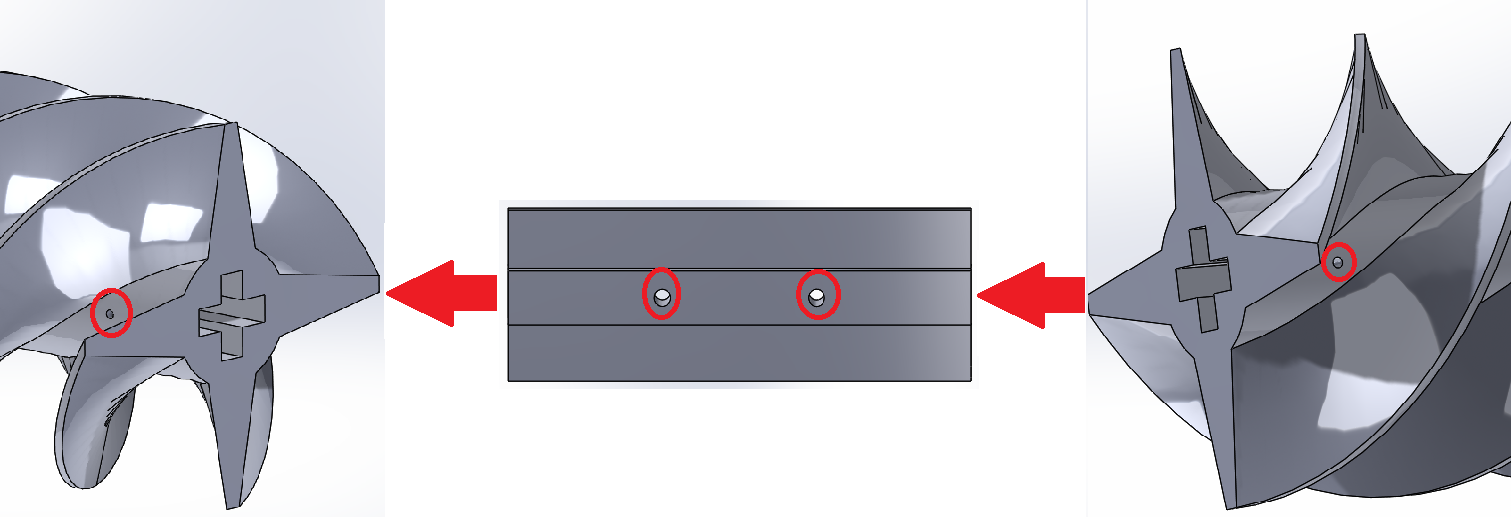
\includegraphics[scale=0.35]{img/ensambletorni.png}
    \end{center}
    \caption{Ensamble del tornillo. \label{ensambletornipng}}
\end{figure}

\subsubsection{Impresión y ensamblaje del tornillo}

El tiempo total requerido para la impresión de las piezas que conforman el tornillo es de aproximadamente 24 horas. Una vez impresas las piezas se obtienen los resultados mostrados en la Figura \ref{piezatornipng}. Debido a que la impresión de piezas 3D se realiza mediante la unión de capas de material derretido, se presentan algunas desviaciones de las medidas deseadas para lo que se debe pulir el resultado con lija; esto se debe realizar especialmente en las áreas de acople para facilitar el ensamble entre las piezas de conexión y las piezas tipo hembra.

    \begin{figure}[H]
        \centering
        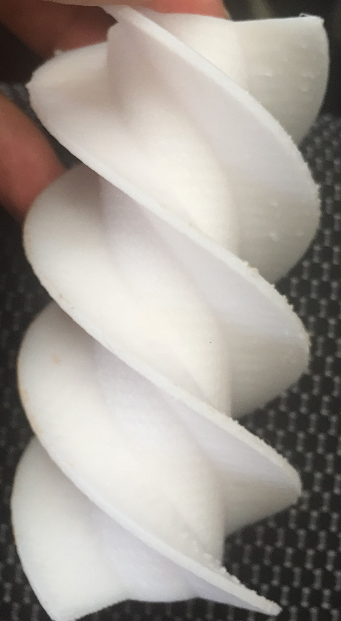
\includegraphics[scale=0.7, angle=90]{img/piezatorni2.png}
        \caption{Ejemplar de pieza impresa del tornillo sin fin} \label{piezatornipng}
    \end{figure}

El proceso de ensamble de las piezas del tornillo es:

\begin{enumerate}[(1)]
    \item Insertar el accesorio circular del servomotor a la pieza del tornillo que cuenta con el empalme correspondiente. Esto se hace mediante los tornillos M3 para unir estas 2 piezas.
    % \begin{figure}
    %     \centering
    %     \includegraphics[scale=0.5]{img/pasostorni1.png}
    %     \caption{} \label{pasostorni1png}
    % \end{figure}
    \item Seguido a esto se debe insertar la pieza de conexión a la ranura de esta primer pieza tipo hembra. Se debe pasar una varilla de $2[mm]$ por medio de los orificios para asegurar el ensamble (Esto aplica para ambos extremos del tornillo)
    %  \begin{figure}
    %     \centering
    %     \includegraphics[scale=0.5]{img/pasostorni1.png}
    %     \caption{} \label{pasostorni1png}
    % \end{figure}
    \item Insertar el extremo restante y ejercer presión hasta que las hélices de ambas partes conformen un único patrón helicoidal.
    %  \begin{figure}
    %     \centering
    %     \includegraphics[scale=0.5]{img/pasostorni1.png}
    %     \caption{} \label{pasostorni1png}
    % \end{figure}
\end{enumerate}

De esta forma se obtiene un tornillo completamente ensamblado como el que se observa en la Figura \ref{tornitotpng}:

     \begin{figure}[H]
        \centering
        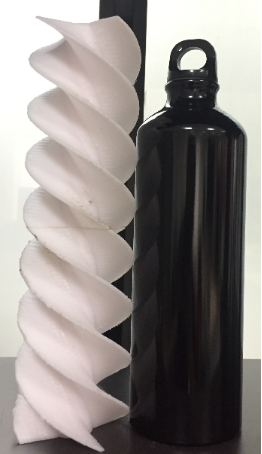
\includegraphics[scale=0.750]{img/tornitot2.png}
        \caption{} \label{tornitotpng}
    \end{figure}

% \textbf{----- Hasta aquí, la parte de implementación del tornillo -----}
\subsection{Unión de partes}

Una vez se tienen todas las partes de la estructura mecánica del prototipo se procede a unirlas para conformar la parte física del mismo. Este proceso se muestra a continuación.

\subsubsection{Parte 1: Estructura Mecánica}

\item \textbf{Tolva, Canalón y Boquilla de descarga}

La tolva tiene una compuerta de entrada en la parte superior y un orificio de salida por donde pasa el alimento de la tolva hacia el canalón (1). Este orificio conecta con la boquilla de entrada del canalón (Orificio vertical de la Tee de PVC, (2)). A su vez, el canalón está conectado con el codo de $90^{o}$  en uno de sus extremos para dar guía de caída del alimento (3), y con el accesorio de limpieza en el extremo restante (4):

\begin{figure}[H]
    \begin{center}
    	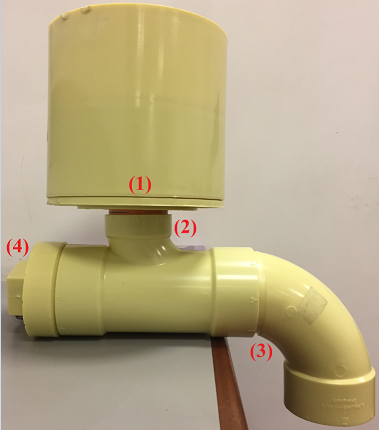
\includegraphics[scale=0.6]{img/tolcancodo2.png}
    \end{center}
    \caption{Unión de la tolva, el canalón y la boquilla de descarga. \label{tolcancodopng}}
\end{figure}

\subsubsection{Parte 2: Dosificación}

\item \textbf{Motor prisionero y Tornillo sin fin}
% Para unir todas las partes que conforman la extracción y dosificación del alimento se deben interconectar las partes encargadas de realizar esta tarea (en cuestión mecánica). Para este prototipo la unión de las partes se hace de la siguiente manera:
De manera simple, la conexión del tornillo ensamblado y el motor aprisionado se hace mediante  el accesorio dentado del motor y un tornillo para asegurarlo al motor. Nuevamente se recalca que este tornillo se introduce en el motor a través del orificio interno que atraviesa el  eje interno del tornillo sin fin. Así pues la unión de esta piezas se observa a continuación:

\begin{figure}[H]
    \begin{center}
    	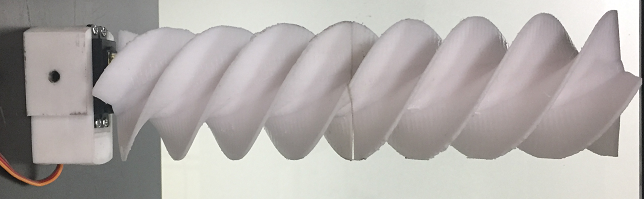
\includegraphics[scale=0.65]{img/tornimotor2.png}
    \end{center}
    \caption{Unión del tornillo impreso y el motor aprisionado. \label{}}
\end{figure}

\subsubsection{Unión de las partes 1 y 2}

Para unir los elementos de las 2 partes ya descritas se debe hacer lo siguiente:

\begin{enumerate}
    \item Separar el canalón, la tolva y  la boquilla de descarga.
        \begin{figure}[H]
            \begin{center}
            	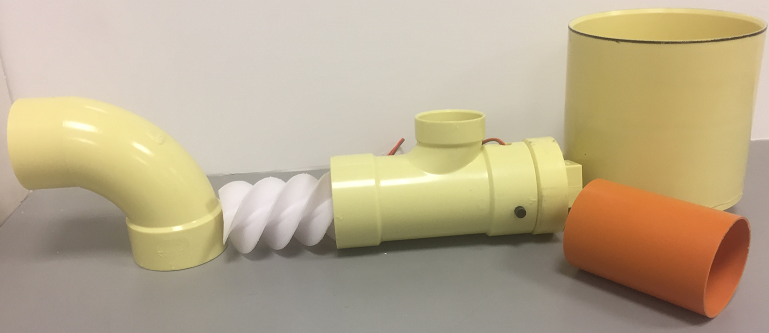
\includegraphics[scale=0.6]{img/separados2.png}
            \end{center}
        \caption{Partes separadas. \label{}}
        \end{figure}
    \item Introducir el motor y el tornillo dentro del canalón de forma que los orificios laterales del canalón estén alineados con los orificios del accesorio de aprisionamiento del motor. De esta forma se garantiza que el accesorio del motor pueda ser aprisionado por los tornillos ubicados en sus costados planos.
        \begin{figure}[H]
            \begin{center}
            	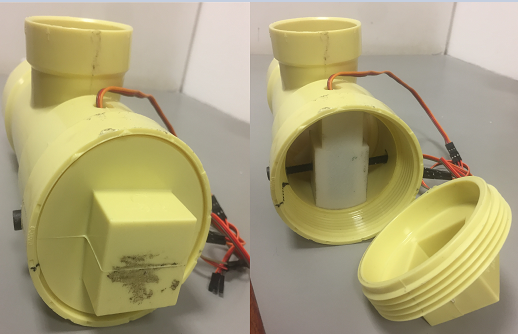
\includegraphics[scale=0.6]{img/ptorni2.png}
            \end{center}
        \caption{Tornillo sin fin y motor, introducidos en el canalón. \label{}}
        \end{figure}
    \item Conectar la tolva y el canalón
        \begin{figure}[H]
            \begin{center}
            	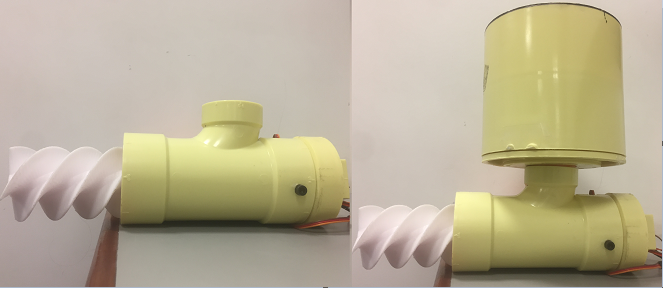
\includegraphics[scale=0.62]{img/ptolva2.png}
            \end{center}
        \caption{Recubrimiento del tornillo. \label{}}
        \end{figure}
    \item Conectar el codo de $90^{o}$ y el canalón mediante la unión de tubería PVC de ventilación (naranja)
        \begin{figure}[H]
            \begin{center}
            	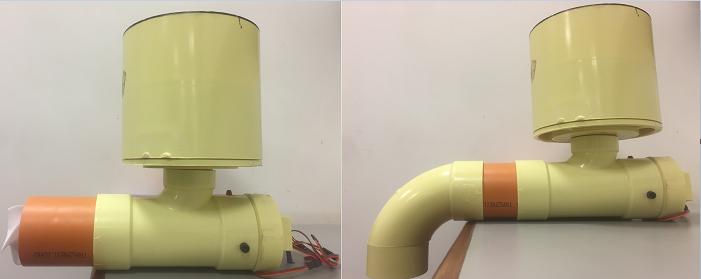
\includegraphics[scale=0.65]{img/pcodo2.png}
            \end{center}
        \caption{Conexión del codo de $90^{o}$. \label{}}
        \end{figure}
\end{enumerate}


\section{Subsistema de Hardware} \label{subsissen}
% \subsection{Sensado}
% \subsubsection{Nivel de alimento de la tolva}
% \subsubsection{RFID}	
% \subsection{Pesaje de alimento / Pesaje de Bovino}
% \subsubsection{Detección de alimento en el comedero}	

\subsection{Actuadores}
% \subsubsection{Motor de giro continuo}
\subsubsection{Accesorio de aprisionamiento del motor (``Suspensor'')}

Teniendo en cuenta la ubicación del motor dentro del canalón mencionada en la Sección \ref{disenotorni} y su orientación horizontal junto con el tornillo dentro del mismo, se requiere de un mecanismo que mantenga fijo al motor para que el torque ejercido pueda hacer girar a la carga y no el efecto contrario. El diseño de este accesorio se describe a continuación:

El motivo principal para incluir esta pieza se debe a que el motor debe poseer una armadura y un soporte que le permita a su eje de giro estar alineado con el eje de giro del tornillo.\\
Sin éste, el motor no podrá transmitir efectivamente el torque. Por su parte, el tornillo puede obstruirse, fragmentarse y en el peor de los casos, romperse debido a la fricción con las paredes del canalón. Así pues, el diseño de este accesorio se describe a continuación:

Para empezar, es indispensable localizar el punto de instalación de este accesorio de suspensión dado que se encontrará en contacto con el motor y por ende dentro del canalón. De esta forma se considera prudente que el accesorio esté asegurado por fricción con las paredes del canalón pero que pueda ser fácilmente removido en caso que se requiera. De esta forma se presupone que el diseño tendrá forma cilíndrica o similar.

\begin{figure}[H]
    \begin{center}
    	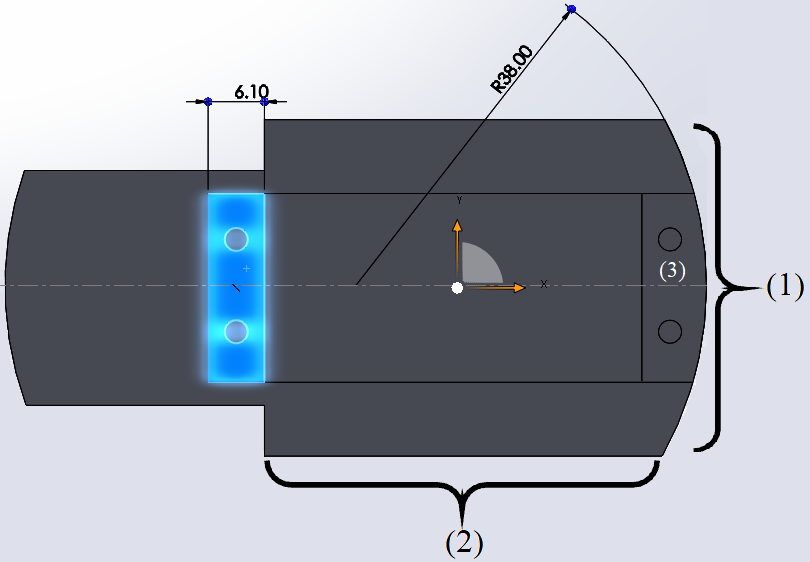
\includegraphics[scale=0.45]{img/suspensorvistasup.png}
    \end{center}
    \caption{Vista superior del accesorio de suspensión.}
\end{figure}

Como se observa en la Figura anterior, las vistas superior e inferior poseen costados de segmentos circulares (1) cuyo diámetro ($76[mm]$), es aproximadamente igual que el diámetro interno del canalón ($76,2[mm]$); así se logra que se mantenga suspendido por fricción.

Los costados planos (2) son pensados para dejar una abertura entre las paredes del accesorio con las paredes internas del canalón y extraer el accesorio junto con el motor y el tornillo. Los cortes internos (3), se deben a las medidas del motor mencionadas en la sección \ref{mg995}; así el motor se fija a éste mediante las salientes del motor que poseen orificios para tornillos M3 (ver corte trasversal en la Figura \ref{cortetrassuspenpng}). 

En esta misma Figura se puede notar un orificio en uno de los costados curvos (4), este orificio es para insertar el motor sin bloquear la conexión con los cables para su uso. También se observa un corte en forma hexagonal junto con un orificio circular (5); este corte se encuentra en ambos lados y esto se añade al diseño para que el accesorio se mantenga fijo por presión. 
La presión es ejercida por 2 tuercas M6 por las que se enroscan 2 tornillos Allen que atraviesan las paredes externas del canalón, se enroscan en las tuercas e imposibilitan deslizamientos involuntarios, indeseados e innecesarios del accesorio. Esto último también se hace para fijar el accesorio en la ubicación correcta dentro del canalón de tal forma que se acople a las medidas del diseño previamente establecido.

\begin{figure}[H]
    \begin{center}
    	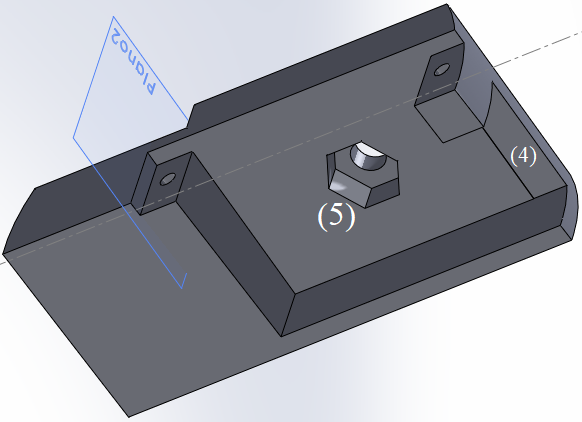
\includegraphics[scale=0.4]{img/cortetrassuspen.png}
    \end{center}
    \caption{Corte trasversal del accesorio. \label{cortetrassuspenpng}}
\end{figure}

Por último, las medidas que complementan el diseño de este accesorio se observan en la Figura \ref{medidassuspenpng}. 

\begin{figure}[H]
    \begin{center}
    	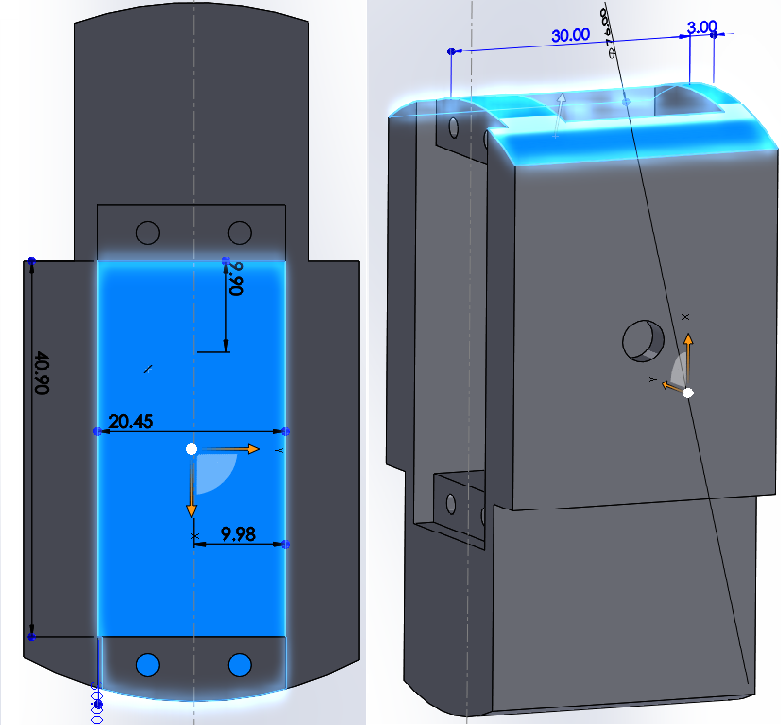
\includegraphics[scale=0.4]{img/otrasmedidassuspensor.png}
    \end{center}
    \caption{Medidas adicionales del diseño del accesorio. \label{medidassuspenpng}}
\end{figure}

Con este diseño finalizado se procede a imprimir esta pieza y a unirla junto con el motor de giro continuo, tal y como se puede ver en la Figura \ref{suspenejpng}.

\begin{figure}[H]
    \begin{center}
    	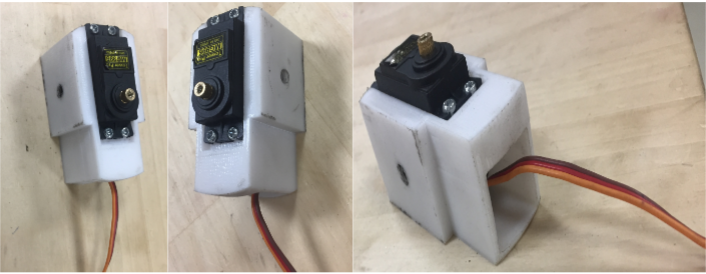
\includegraphics[scale=0.9]{img/suspenej2.png}
    \end{center}
    \caption{Unión entre el motor y el accesorio de aprisionamiento. \label{suspenejpng}}
\end{figure}

Seguido a este se inserta esta unión dentro del canalón para verificar que éste pueda ser debidamente aprisionado y se mantenga fijo durante su accionamiento. Para esto se muestran diferentes puntos de vista en la Figura a continuación:

\begin{figure}[H]
    \begin{center}
    	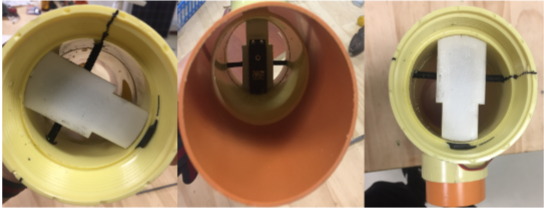
\includegraphics[scale=0.95]{img/prisionero2.png}
    \end{center}
    \caption{Aprisionamiento del motor del tornillo dentro del canalón. \label{prisioneropng}}
\end{figure}

\subsection{Extracción de alimento asociado al novillo}

Para satisfacer de manera experimental el objetivo específico \#2, la extracción del alimento acorde a un novillo determinado se logra al manipular el tornillo sin fin y una báscula de pesado cuyo límite está definido por el valor asociado a la etiqueta RFID que posea el novillo en su jáquima. Los elementos usados son el ADC HX711 conectado a la celda de carga de la báscula, el servo de giro continuo que acciona al tornillo conectado con una fuente de alimentación y el arduino para la señal de control, y por último la conexión entre el ADC HX711 y el arduino. Dichas conexiones se indican en la Tabla \ref{conexfood}.

\begin{table}[H]
\centering
\caption{Conexión entre componentes usados para la extracción, verificación y validación de las porciones dietarias.}
\label{conexfood}
\begin{tabular}{|
>{\columncolor[HTML]{FFFFC7}}c |cccc|c|l|lc|l|l|}
\hline
ADC HX711                         & E+   & E-    & A-    & A+     & \multicolumn{3}{c|}{\cellcolor[HTML]{34CDF9}Arduino} & \multicolumn{3}{c|}{\cellcolor[HTML]{34CDF9}Tornillo} \\ \cline{2-11} 
Celda de carga (Báscula)          & Rojo & Negro & Verde & Blanco & \multicolumn{3}{c|}{5V}                              & \multicolumn{3}{c|}{Rojo}                             \\ \cline{1-5}
\cellcolor[HTML]{67FD9A}ADC HX711 & GND  & DT    & SCK   & VCC    & \multicolumn{3}{c|}{GND}                             & \multicolumn{3}{c|}{Cafe}                             \\ \cline{2-5}
\cellcolor[HTML]{67FD9A}Arduino   & GND  & A1    & A0    & 5V     & \multicolumn{3}{c|}{Pin 3}                           & \multicolumn{3}{c|}{Naranja}                          \\ \hline
\end{tabular}
\end{table}

%%% Tek: sigo sin entender las coenxiones en la Tabla

% \begin{table}[H]
% \centering
% \begin{tabular}{|c|cccc|c|l|lc|l|l|}
% \hline
% HX711   & E+   & E-    & A-    & A+     & \multicolumn{3}{c|}{Arduino} & \multicolumn{3}{c|}{Tornillo} \\ \cline{2-11} 
% Báscula & Rojo & Negro & Verde & Blanco & \multicolumn{3}{c|}{5V}      & \multicolumn{3}{c|}{Rojo}     \\ \cline{1-5}
% HX711   & GND  & DT    & SCK   & VCC    & \multicolumn{3}{c|}{GND}     & \multicolumn{3}{c|}{Café}     \\ \cline{2-5}
% Arduino & GND  & D3    & D2    & 5V     & \multicolumn{3}{c|}{Pin 3}   & \multicolumn{3}{c|}{Naranja}  \\ \hline
% \end{tabular}
% \caption{Conexiones para la extracción, verificación y validación de las porciones dietarias.}
% \label{conexfood}
% \end{table}

Una vez hechas las conexiones pertinentes, el programa ejecutado ofrece los siguientes resultados.
\begin{enumerate}
    % \item La gramera digital posee un factor de calibración de -455188; gracias a este valor el dispositivo ADC HX711 (usado con la gramera) permite medir valores en [g] con variación de hasta $\pm 0.5[g]$.
    \item El valor que mide la gramera puede ser promediado por un número determinado de muestras. Entre mayor cantidad de muestras requeridas, más lenta es la ejecución del programa pero la medición lograda suele ser más precisa.
    \item Mientras que el peso de la gramera no sea igual o superior al peso determinado por el valor \texttt{Diet[j]}, el servo que acciona el tornillo sin fin, extraerá alimento desde el tanque.
    \item Una vez el peso supere el valor de la dieta, el tornillo deja de girar, y se da paso a la entrega del alimento hacia el plato.
    \item La gramera no dejará de medir el peso hasta que su nuevo peso sea aproximadamente igual a cero. Una vez esto sucede, procedemos a analizar la verificación de comida en el plato y se da paso a la etapa de ingerir el alimento
    \item Para más detalles ver observaciones de colores de la Figura \ref{resgramerapng}.
\end{enumerate}

\begin{figure}[H]
    \begin{center}
    	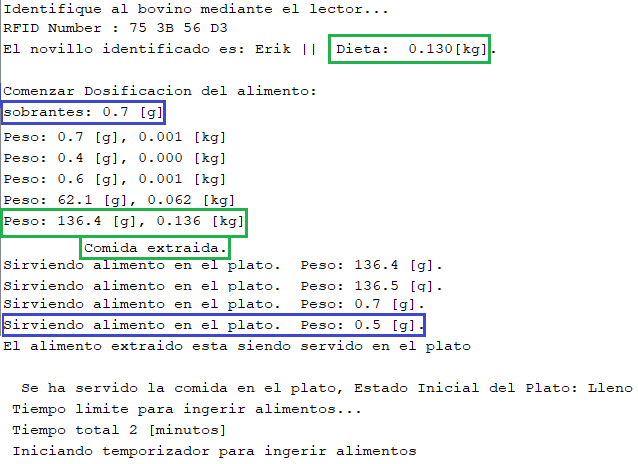
\includegraphics[scale=0.7]{img/resgramera.png}
    \end{center}
    \caption{Resultados de la extracción y pesado del alimento.} \label{resgramerapng}
\end{figure}

Nótese de la Figura anterior que cuando el valor de la gramera supera el valor de la dieta (cuadro verde), se da aviso exitoso de la extracción del alimento. Esto a su vez detiene el accionamiento del tornillo. Seguido a esto la gramera deja de estar en funcionamiento cuando su valor medido se aproxime a cero o a un valor restante ocasionado por sobras que deja el alimento sobre la superficie de la misma (cuadro azul). Finalmente cuando esto sucede, se da paso a la detección de alimento en el plato, y a la etapa de consumo del alimento.
% \begin{figure}[H]
% 	\begin{center}
% 		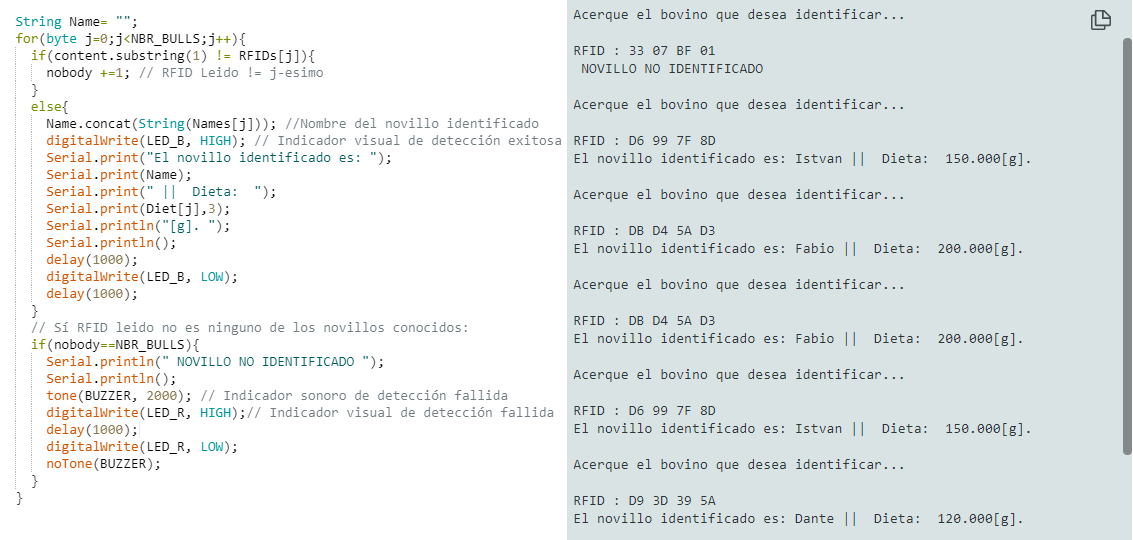
\includegraphics[scale=0.55]{img/cmdrfid.png}
% 	\end{center}
% 	\caption{Código y ejecución del programa de identificación de novillos.}
% \end{figure}

\subsection{Entrega de alimento hacia el plato}\label{biela}

El objetivo específico \#3 indica que el alimento extraído y pesado en la gramera será servido en el plato mediante un mecanismo de dosificación. Para satisfacer con este objetivo se había pensado en el uso de las escobillas descritas en la sección \ref{escobillas}. No obstante, la aplicación práctica de este mecanismo requería de una sincronización de los motores actuadores mediante un sistema mecánico de cadenas y poleas que superaron las limitaciones del proyecto. Como medida correctiva se optó por utilizar un mecanismo de Biela-Manivela. De esta forma el alimento sería desplazado linealmente aún cuando se utilizase el movimiento rotativo del motor actuador.

\begin{figure}[H]
	\begin{center}
		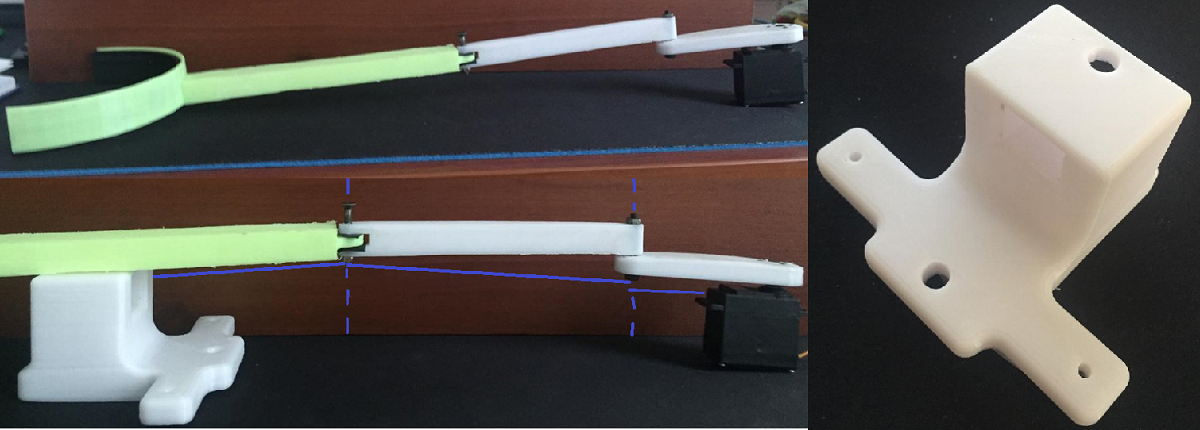
\includegraphics[scale=0.50]{img/manivela.png}
	\end{center}
	\caption{Mecanismo de Biela-Manivela utilizado.}\label{manivela}
\end{figure}

Sin embargo, aún cuando este mecanismo fue diseñado, fabricado y puesto en práctica (ver Figura \ref{manivela}), debido a falencias en el material de impresión, la longitud de la biela y de la manivela causan una curvatura en el material que impide un correcto alineamiento entre las partes y hace que las articulaciones no puedan transmitir el movimiento satisfactoriamente dificultando su aplicación en el proyecto. Esta desalineación entre la biela y la manivela hace que el riel guía no esté a la altura requerida para guiar al extremo verde que empujaría la comida. Además la curvatura de las piezas genera una fricción indeseada que afecta la transmisión de torque por parte del motor ocasionando que realice movimientos o traslaciones bruscas de una posición a otra.

Lastimosamente, este objetivo no puede ser realizado satisfactoriamente debido a que la situación social ocasionada por la pandemia del COVID-19 no posibilita el acceso a las herramientas necesarias que permitan una adaptación o nueva fabricación del mecanismo. De esta manera la realización de este objetivo se concluye como no viable en la situación actual.

\subsubsection{¿Medidas correctivas o posibles soluciones?}

Bajo condiciones normales o de libre acceso a herramientas de trabajo pertinentes se podría optar por las siguientes medidas correctivas:
\begin{enumerate}
    \item Reconstruir las piezas de la Biela y la Manivela con una estructura interna más concentrada de material de impresión 3D y verificar que la cama de impresión se está calentando correctamente.
    \item Construir las piezas de la Biela y la Manivela con materiales más robustos como plástico o aluminio.
    \item Fabricar un riel de guía de una longitud igual al brazo de color verde (ver Figura \ref{manivela}), o sea, el extremo que empuja el alimento de forma lineal.
    \item Posicionar el mecanismo de la Biela-manivela sobre una superficie deslizante que coincida con la altura de la superficie de la báscula donde se pesa la comida. De esta forma el extremo verde se deslizaría alternando entre la superficie de guía y la superficie de la báscula.
    \item Modificar las articulaciones de conexión o utilizar arandelas que ayuden a nivelar las deficiencias entre la biela y la manivela.
    \item Aumentar el largo de la manivela o el ancho del brazo de color verde.
\end{enumerate}

\subsection{Temporizador y verificación de alimento en el plato}

Para satisfacer de manera experimental el objetivo específico \#5 se debe corroborar si un novillo ha ingerido su alimento. Esto se logra mediante una detección electrónica utilizando sensores infrarrojos tal y como se mencionó en la sección \ref{detectcomedero}. 

Los resultados obtenidos indican dos cosas. La primera es una detección inicial del alimento en el momento en que este último se desplaza de la gramera hacia el plato. La segunda es una detección final que se lleva a cabo al finalizar el tiempo de consumo de alimento (Ver Figura \ref{comidaplatopng}).

Si el estado inicial coincide con el estado final, el alimento no habrá sido consumido y por lo tanto se debe registrar este evento en la base de datos. En caso contrario, el consumo del alimento es exitoso y se registra en la base de datos. Con la intención de lograr un resultado más informativo, se ha clasificado el plato por niveles para indicar qué tanto se ha ingerido desde el estado inicial. Con esto se permite identificar falencias en el consumo con un cierto grado de alarma.

\begin{figure}[H]
	\begin{center}
		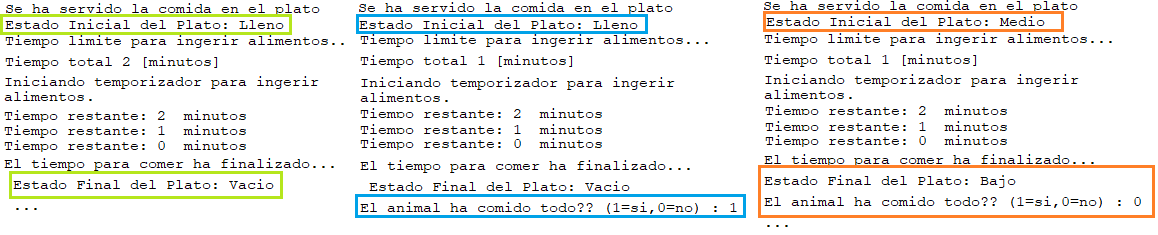
\includegraphics[scale=0.54]{img/comidaplato.png}
	\end{center}
	\caption{Detección de consumo del alimento en el plato.}\label{comidaplatopng}
\end{figure}

 En la parte izquierda de la Figura anterior se observa una detección de alimento servido en el plato indicando su estado inicial y su estado final. Aún cuando esto es suficiente para corroborar la existencia de alimento servido en el plato se opta por agregar una consideración más informatica a esta validación. En la parte derecha de la Figura \ref{comidaplatopng}, se observa que aún cuando el nivel del plato disminuyó de Medio a Bajo (hubo consumo del alimento), este consumo no fue completo lo que permite detallar un poco más este tipo de situaciones.

%%% Tek informatica?

\subsection{Pesaje del novillo}

En pro de satisfacer el objetivo específico \#7, se utiliza un arreglo de puente completo de Wheatstone, lo que permite medir pesos mayores a comparación del arreglo usado con la gramera digital. En este caso, la medición del peso se detiene mediante la pulsación de un botón. De esta manera se puede almacenar el peso una vez que este converja en un valor más preciso. Los resultados del programa permiten obtener lo siguiente:

\begin{figure}[H]
	\begin{center}
		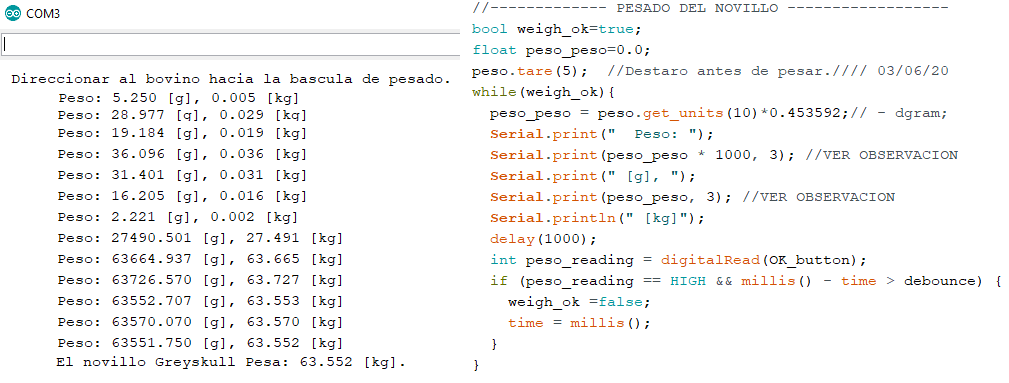
\includegraphics[scale=0.57]{img/pesobovino.png}
	\end{center}
	\caption{Pesaje del bovino.}\label{pesobovinopng}
\end{figure}
% \pagebreak

\subsection{Verificación de alimento suficiente en el tanque}

De acuerdo con el objetivo específico \#1, se debe realizar una comprobación de alimento suficiente en el tanque de almacenamiento para dar abasto a futuros individuos. Este objetivo se logra al utilizar una variable acumuladora que, como su nombre lo indica, acumula los valores extraídos del tanque y los substrae de la cantidad máxima del tanque, esto  puesto que las pruebas se basan en ``el peor de los casos'' (ver sección \ref{lvltolva}).

En la parte derecha de la Figura \ref{lvltanquepng} se puede evidenciar la parte de código encargado de activar una alarma sonora y una alarma visual, en caso tal que el alimento en el tanque (Objetivo específico \#1) no sea mayor a la cantidad mínima requerida. Con base en lo anterior, se concluye que el objetivo específico\#8 se satisface por esta condición.\\

\begin{figure}[H]
	\begin{center}
		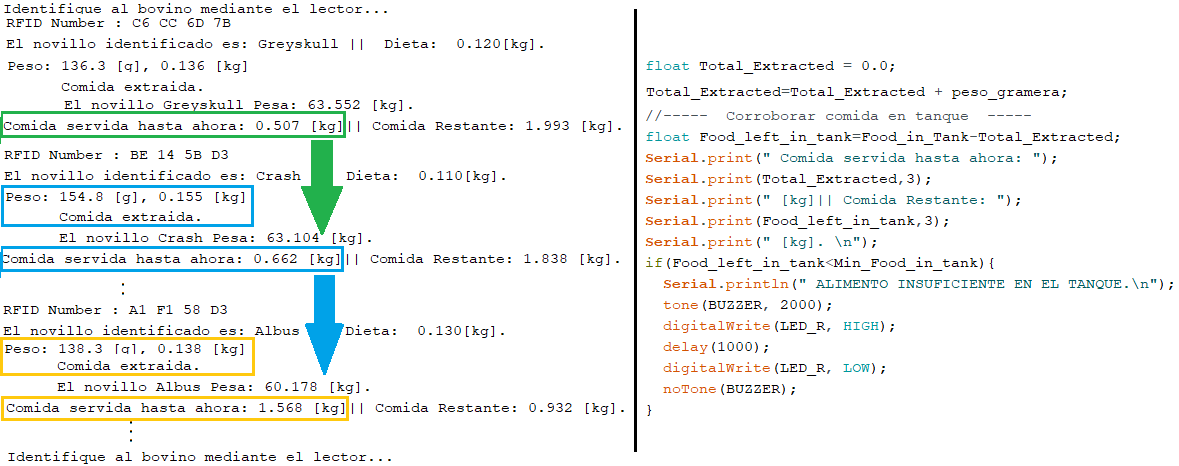
\includegraphics[scale=0.53]{img/lvltanque.png}
	\end{center}
	\caption{Comprobación de alimento en el tanque.}\label{lvltanquepng}
\end{figure}

\subsection{Esquema final de conexiones}

Una vez se han realizado las conexiones pertinentes entre los dispositivos usados en cada una de las etapas, se obtiene un esquema de conexiones como el de la Figura \ref{esquemafinalpng}. En orden, de izquierda a derecha en la figura, los dispositivos usados son los siguientes:

\begin{multicols}{2}
    \begin{itemize}
        \item Módulo $\mu$SD (x1) \item Lector RFID (x1) 
        \item Detector Infrarrojo (x3) \item ADC HX711 (x2)
        \item Celda de carga (x2) \item Protoboard (x2)
        \item $\mu$C Arduino Mega (x1) \item Servo MG995 (x2)
    \end{itemize}
\end{multicols}
    
\pagebreak

\begin{figure}[H]
	\begin{center}
		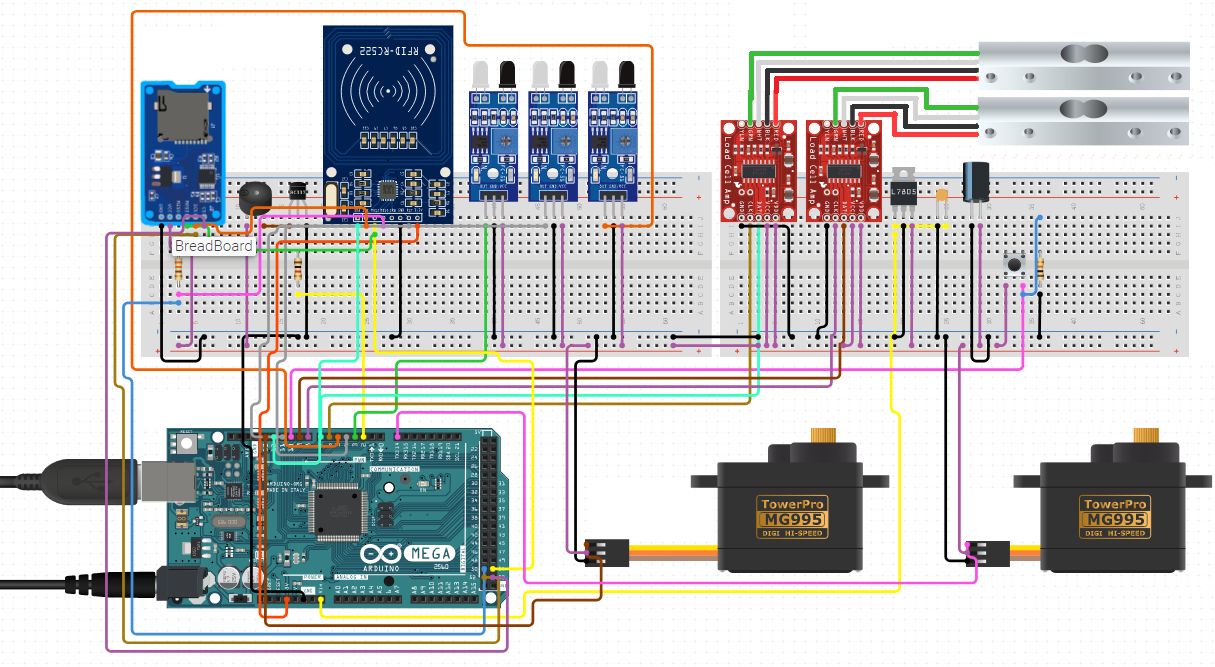
\includegraphics[scale=0.64, angle=90]{img/Full_Schematic.png}
	\end{center}
	\caption{Esquema final de conexiones entre dispositivos}\label{esquemafinalpng}
\end{figure}


%%% Tek segmento de código?---la parte de código --> Corregido



% \pagebreak

\section{Subsistema de procesamiento de datos}

%% Objetivos 6 , 9 , 10  y 11
\subsection{Resultados de almacenamiento de datos} \label{datosinteres}

Llegados a este punto se tiene la ejecución del sistema de manera eficaz, esto quiere decir que todas las partes cumplen con la función para las que fueron diseñadas; de esta manera solo resta almacenar los datos que se adquieren en las iteraciones diarias del ciclo de ceba.\\

Los datos que se han establecido como datos de interés son los siguientes:\\

\begin{enumerate}
    \item \texttt{Nom}: El nombre del bovino que ingresa a la iteración \texttt{n}-ésima de la ejecución del sistema, con $\texttt{n = 1, 2, 3, \ldots}$
    \item \texttt{Diet}: La porción de alimento dietario correspondiente al bovino \texttt{n}-ésimo.
    \item \texttt{IDal}: Variable que indica la activación de alarma en el subsistema de Identificación por motivo de novillo no identificados.
    \item \texttt{IDrep}: Variable que indica la activación de alarma en el subsistema de Identificación por motivo de novillos que intentan repetir su alimentación. 
    \item \texttt{Vextract}: Valor final de alimento extraído por el tornillo y pesado en la báscula digital una vez éste supere el valor \texttt{Diet}.
    \item \texttt{extract}: Indicador de extracción exitosa de alimento para el novillo \texttt{n}-ésimo.
    \item \texttt{Served}: Variable de código para corroboración de alimento servido en el plato para el novillo \texttt{n}-ésimo.
    \item \texttt{Fonplate}: Indicador de validación de alimento en el plato para el novillo \texttt{n}-ésimo.
    \item \texttt{Plate\_s}: Estado inicial del plato una vez se haya servido alimento en él.
    \item \texttt{Plate\_f}: Estado final del plato al finalizar el temporizador.
    \item \texttt{Eatenal}: Variable que indica la activación de alarma en la etapa de consumo de alimento en caso tal que no se ingiera la totalidad del alimento.
    \item \texttt{Eaten}: Variable de código para indicar el consumo total de alimento.
    \item \texttt{Peso}: Variable que representa el peso del novillo \texttt{n}-ésimo
    \item \texttt{Tankal}: Variable que indica la activación de alarma en caso tal que el alimento en el tanque se encuentre por debajo de la cantidad mínima sugerida.
\end{enumerate}

%%% Tek: la extensión convencional para esto es csv (comma-separated values: https://en.wikipedia.org/wiki/Comma-separated_values) y, claro el separador es la coma. También puede ser character-separated values, en cuyo caso, el separador podría ser el punto y coma

Una vez que la iteración \texttt{n}-ésima haya finalizado, los datos previamente descritos, son almacenados en un archivo plano de texto (\texttt{*.txt}) y se encontrarán separados por un ``punto y coma'' (\texttt{;}).
Cada uno de los \texttt{m}-renglones que se registren en este archivo representan los datos de interés de los \texttt{m}-novillos que han pasado por la iteración de alimentación planteada en este proyecto. Dentro de estos se incluyen las situaciones en las que se presenten novillos no identificados o que intenten repetir.
Así pues, los datos que se tendrán registrados en un archivo de texto para una prueba del sistema podrán observarse en el lado izquierdo de la Figura \ref{sdtxtpng}.
Para mayor comodidad, estos datos pueden ser re organizados y representados por matrices en archivos de Excel tal y como se muestra en lado derecho de la Figura \ref{sdtxtpng}, lo que posibilita un análisis de datos mediante gráficos, filtros y otros complementos.

% \pagebreak

\begin{figure}[H]
	\begin{center}
		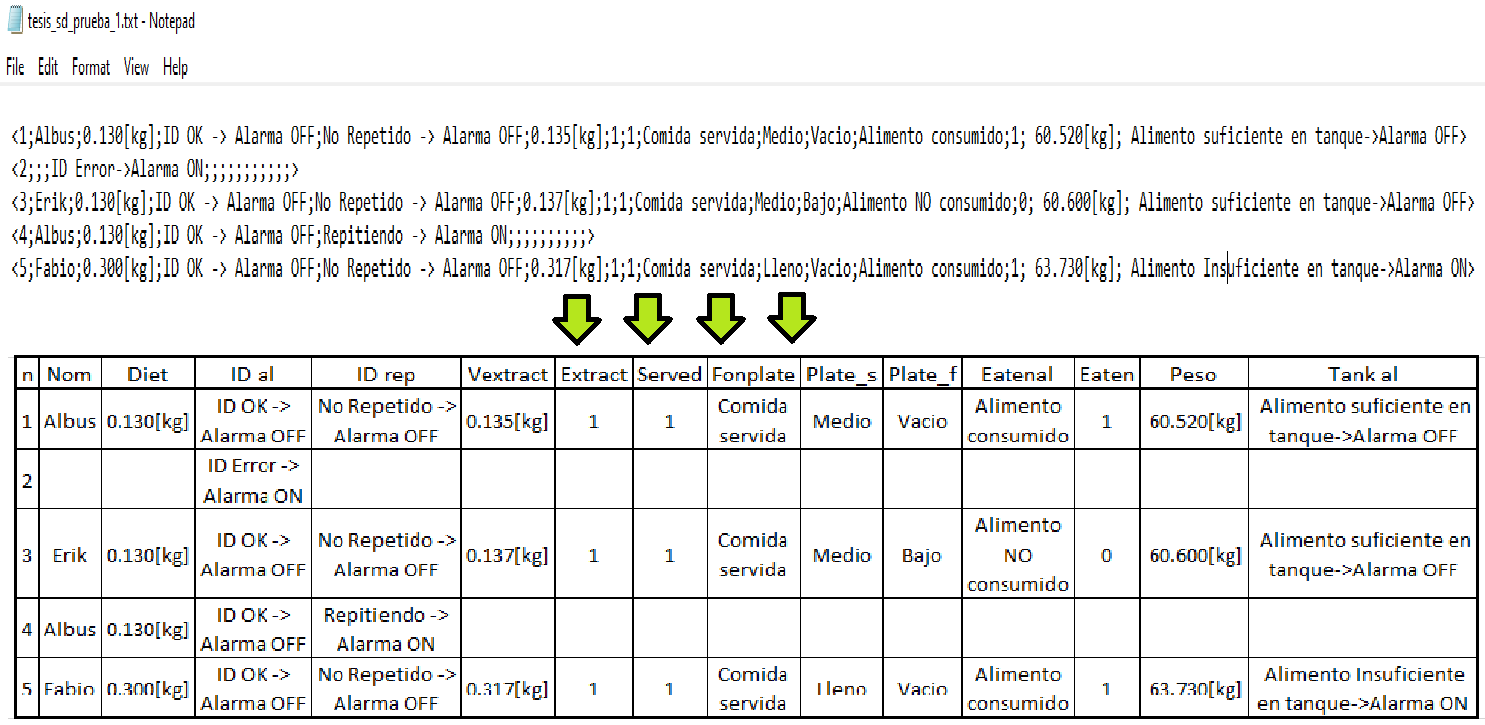
\includegraphics[scale=0.52,angle=90]{img/sdtxt.png}
	\end{center}
	\caption{Ejemplo de archivo de texto y tabla de Excel generados con los datos registrados.}\label{sdtxtpng}
\end{figure}

% \begin{figure}[H]
% 	\begin{center}
% 		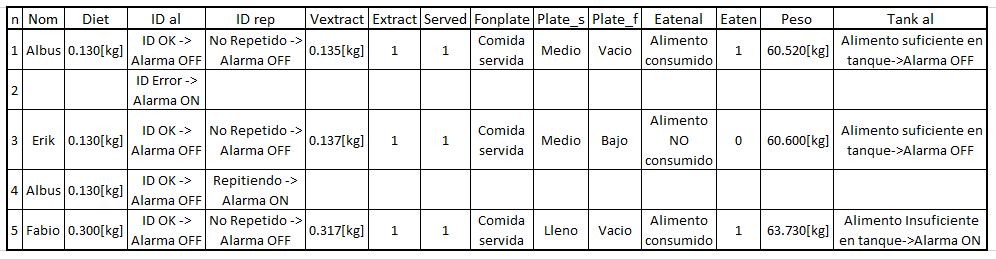
\includegraphics[scale=0.6]{img/sdexcel.png}
% 	\end{center}
% 	\caption{Ejemplo de archivo de excel con base en el archivo txt de la Figura \ref{sdtxtpng}}\label{sdtxtpng}
% \end{figure}

%  05/06/20  Esto que esta comentado ya no va, no lo borro hasta que el doc quede aprobado por el profe
%  Regla #1 de la electrónica, si esta funcionando, no lo toques xD

% \subsubsection{Sistema de Alarmas}
% \subsection{Microcontrolador}

% \subsection{Composición mecánica de un punto de alimentación}

% \textbf{Hablar z poner algo de la Figura de unionespvc total la debo poner en los resultados del sistema mecánico. y eso seria como todo el esquema de la unión de todas las partes.}
